\section{Augmenting the MESA Grid}\label{sec:augmentation}

With the GP model described in Section \ref{GPR},  we train GP models for the MESA grid. The training data includes the primary and the additional girds as mentioned in Table~\ref{tab:grid}. The role of the additional grid is increasing the grid resolution for the high-mass models with hooks. As discussed in the previous section, the kernel function in the 'hook' area are much more complex than other regions , and hence a GP model requires more information to map the feature in this region. The total training data includes $\sim$ 15,000 evolutionary tracks and $\sim$ 10,000,000 data points. For validating and testing the data, we computed another 4880 tracks with random model inputs within the grid ranges. These tracks are split 50-to-50 for validating (in the training progress) and testing (after the training progress) GP models. We used the same sampling method of training, validating, and testing data. For each EEP section, we use 20,000 training data points and 20,000 validating data in the training progress.The testing data are selected in the whole EEP range and we use 50,000 (out of $\sim$1,000,000) data points. Note that we do not use models with $\tau \geq$ 20.0 Gyr, [Fe/H]$_{\rm surf} \leq$ -0.6 dex, or $T_{\rm eff} \geq$ 7000$K$ as testing data.    

\subsection{Overall Results}

We firstly train an Exact GP model for the whole grid with 20,000 model, corresponding to a sampling rate of $\sim$0.2\%. The testing indexes of outputs remarkably increase compared to those of 3D GP models. We listed the testing errors of this 5D GP model in Table~\ref{tab:results}. Results of 2D and 3D GP models are also given for comparisons. It shows clear decline in GP model accuracy with increasing input demission. 
%
We then train GP models with the section scenario. We gradually increase the number of sections and track changes in testing errors. We found that improvements in testing errors becomes not significantly when the section number goes above 10. As it shown in Table~\ref{tab:results}, the 68th and 95th testing errors are at same accuracy levels for sections more than 10. Although the 99.7th errors seem to be better with more sections, this is more like a random error given the change is a small fraction. 
%
It turns out that the most efficient sampling rate is around 1\% (10 sections). Above this rate, GP models learn no additional information about the grid.  
%
We take the 10-sections GP model as the final solution. Following analysis are all done with this model.   


\begin{table*}
	\centering
	\caption{Training and validating errors for GPR Models}
	\label{tab:results}
	\begin{tabular}{cccccccccc}
		\hline
		Model Type&Inputs&$N_{\rm Training}$ &Sampling rate &\multicolumn{5}{c}{Testing Errors (at 68/95/99.7\%)} \\
		 \hline
		 \multicolumn{4}{c}{}& $T_{\rm eff}$ &$\log g$  &$R$  &[Fe/H]$_{\rm surf}$   &$\tau$ \\
		 \multicolumn{4}{c}{}&  (K)& ($10^{-3}$dex) & ($10^{-3}R_{\odot}$)  &  ($10^{-3}$dex)  & ($10^{-2}$Gyr) \\		 
		 \hline
		 Exact GP & 2D & 20,000 x 1 &96\% & 1/5/11 & 1/3/8 & 2/6/14 & 0.5/2/12 &  1/3/9 \\
		 %SVGP & 2D & 2,000 x 10  &96\% & 1/5/11 & 1/4/10 & 3/7/14  & 0.3/2/14 & 1/4/10  \\
		 \hline		 
		 Exact GP & 3D & 20,000 x 1 & 5\% & 2/6/16 & 1/4/10 & 3/7/17 &  2/6/22 & 2/7/22 \\
		 %Exact GP (5 sections) & 3D & 20,000 x 5 & 20\% & 2/6/17 &1/4/10 & 3/7/16& 1/3/18& 2/6/19\\
		  Exact GP (10 sections) & 3D & 20,000 x 10 & 50\% & 2/5/15 &1/4/11 & 2/7/17& 1/3/20& 2/6/19\\
		% SVGP (too slow) & 3D & 2,000 x 50 & 25\% & 3/7/16 & \\
		 %SVGP (too slow)  & 3D & 5,000 x 20 & 25\% & 2/7/15 & & & & & \\
		 %GIGP (Relu + normal data)& 3D & 100K & 25\% & 2/7/14  & & & & & \\
		 %GIGP (Relu + normal data)& 3D & 200K & 50\% & 4/8/17  & & & & & \\
		 %GIGP (Relu + grid data)& 3D & 220K & 50\% & 5/10/28 & & & & & \\
		 %GIGP (elu + grid data)& 3D & 220K & 50\% & 7/12/29 & & & & & \\
		 %\hline
		 %Exact GP (multitask) & 3D & 20,000 x 1 & 5\% & memory  &  &  &   &  \\
		  \hline		 
		 Exact GP & 5D & 20,000 x 1 & 0.2\% & 3/9/34 & 2/5/18 & 4/11/36 & 2/7/30 & 3/9/27  \\
		 Exact GP (3 sections) & 5D& 20,000 x 3 & 0.6\% &  3/8/27 & 2/5/18 & 3/7/26 & 1/4/24 &3/7/22 \\
		 %Exact GP (3 sections) & 5D& 20,000 x 3 & 0.6\% &  2.5/7.7/27.4 & 15/45/177 & 26/73/257 & 9/42/236 &26/73/226 \\
		 Exact GP (5 sections) & 5D& 20,000 x 5 & 1\% &  2/7/25 & 1/4/15 & 3/7/24 & 1/4/21 &2/6/22 \\
		 %Exact GP (5 sections) & 5D& 20,000 x 5 & 1\% &  2.4/7.2/24.8 & 13/39/152 & 25/71/242 & 9/39/207 &21/64/215 \\
		 Exact GP (10 sections) & 5D& 20,000 x 10 & 2\% & 2/7/27  & 1/4/14 & 2/7/26 &1/4/20 & 2/6/21\\
		 %Exact GP (10 sections) & 5D& 20,000 x 10 & 2\% & 2.4/7.1/26.8  & 14/40/141 & 24/70/263 &9/37/196 & 21/64/208\\
		 Exact GP (20 sections) & 5D& 20,000 x 20 & 4\% & 2/7/26  & 1/4/14 & 2/7/27 &1/3/18 & 2/6/22 \\
		 %Exact GP (20 sections) & 5D& 20,000 x 20 & 4\% & 2.2/6.9/26.1  & 13/38/141 & 24/72/290 &9/32/182 & 19/61/218 \\
		  Exact GP (100 sections) & 5D& 20,000 x 100 & 20\% & 2/7/25  & 1/4/14 & 2/7/26 &1/3/17 & 2/6/18 \\
		 % Exact GP (100 sections) & 5D& 20,000 x 100 & 20\% & 2.2/6.7/25.8  & 13/36/157 & 23/67/283 &8/34/185 & 19/59/190\\
		 %GIGP (Elu) & 5D & 10 x10,000 & 1\% & 5/12/34 & & & & \\
		 %GIGP (Relu) & 5D & 10 x10,000 & 1\% & 6/13/47 & & & & \\
		 %GIGP & 5D &  & 2\%, 5\%, 10\%, 25\%  & memory & & & & \\
		% \hline
		 % \multicolumn{9}{c}{GP a subset of 5D data-hook}\\
		 %\hline
		 %Exact GP EEP = 0.2-0.4 & 5D & 20,000 x 1 & 1\% & 2/7/20 &&&\\
		 %Exact GP EEP = 0.3-0.4 & 5D & 20,000 x 1 & 2\% & 3/8/21  &&&\\
		 %Exact GP EEP = 0.3-0.35 & 5D & 20,000 x 1 & 3\% & 2/7/17 &&&\\
		  %Exact GP EEP = 0.3-0.32 & 5D & 20,000 x 1 & 8\% & 2/5/14 &&&\\
		 %Exact GP EEP = 0.3-0.31 & 5D & 20,000 x 1 & 16\% & 2/4/13  &&&\\
		  \hline
	\end{tabular}
\end{table*}


We show the testing errors in Figure~\ref{fig:5d_test_vs_input}. 
%
Because of the tail feature as illustrated in Figure~\ref{fig:2dtest}, 95\% confidential intervals vary in larger dynamic ranges than 68\% confidential intervals.  
%
Testing errors of $T_{\rm eff}$, $\log g$, and $R$ mainly depend on $M$ and $EEP$. Metallicity error strongly depends on $M$, $EEP$, and [Fe/H]$_{\rm init}$, and age error has a significant correlation to $EEP$ and [Fe/H]$_{\rm init}$. However, testing errors do not obviously relate to $Y_{\rm init}$ or $\alpha_{\rm MLT}$. 

\begin{figure*}
	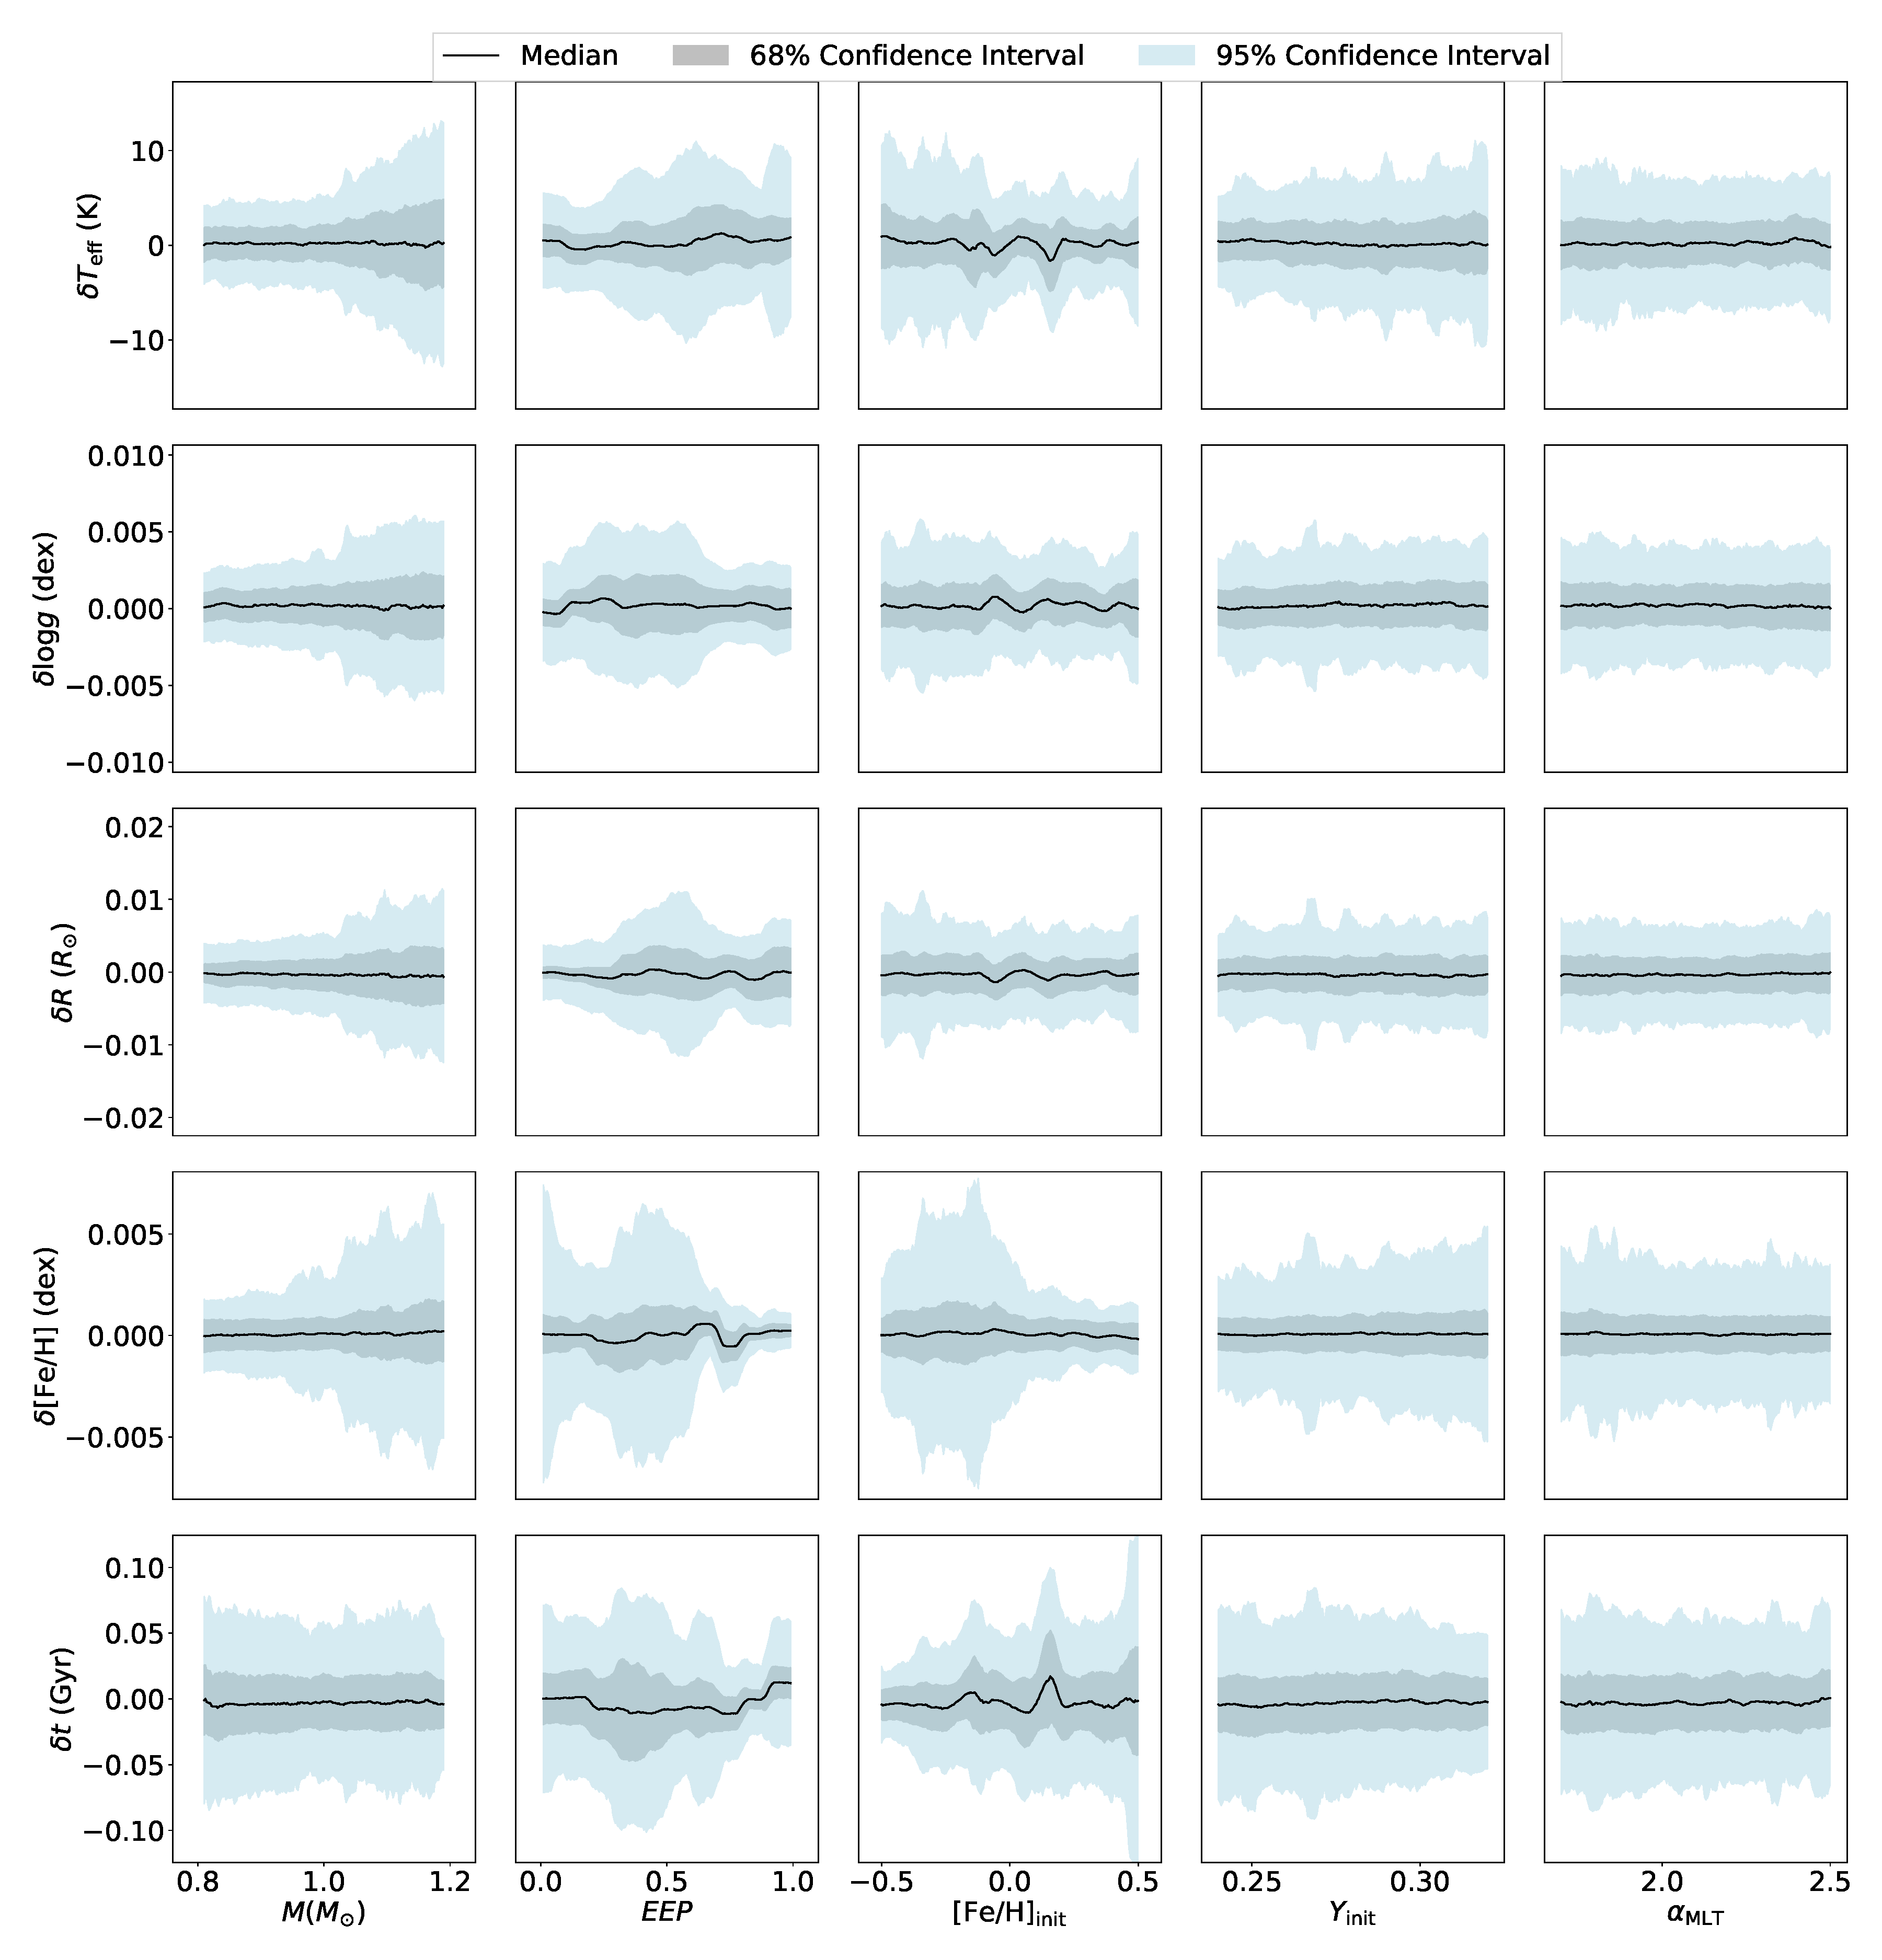
\includegraphics[width=2.0\columnwidth]{ 5d-testing_vs_inputs.pdf}
    \caption{ Roll medians and confidential interval of testing errors against GP model  inputs. Black solid line indicate the median; grey and blue shadow represent the 68\% and 95\% confidential interval. Testing errors of $T_{\rm eff}$, $\log g$, and $R$ mainly depend on $M$ and $EEP$. Metallicity error strongly depends on $M$, $EEP$, and [Fe/H]$_{\rm init}$, and age error has a significant correlation to $EEP$ and [Fe/H]$_{\rm init}$. However, testing errors do not obviously relate to $Y_{\rm init}$ or $\alpha_{\rm MLT}$. } 
  \label{fig:5d_test_vs_input}
\end{figure*}

\subsection{Mapping Systematical Uncertainties across the input parameter space}\label{sec:sys}

Local standard deviations are not uniform and correlate to multiple inputs and hence marginal values in Figure~\ref{fig:5d_test_vs_input} do not properly describe systematical uncertainties of GP model.  
% 
Because marginal values do not obviously relate to $Y_{\rm init}$ or $\alpha_{\rm MLT}$. A comprehensive statistical model for systematical uncertainty can be described as a function of $M$, $EEP$, and [Fe/H]$_{\rm init}$. 
%
We first examine local error distributions across this 3-demissions input space. This is to investigate wether local testing errors form the Gaussian function (without tails). We divided the input space into equal-size segments. Note that the the choice of the size matters. It needs to be small enough to present the local feature. However, it can not be very small so that there are not enough data points for statistical analysis. 
%
We divide the input range into 40 equally spaced segments for $M$, 20 for [Fe/H]$_{\rm init}$, and 25 for $EEP$. The 3D parameter space is hence divided into 20,000 cubes. For each cube, we calculate rolling median value and standard deviation in the 3D space with the data in this cube and other 26 cubes around it. 
%
In the computation, we do a statistic test to ensure the local error distribution has no tail effect. Two conditions are used for the test. One is the 68\% CI over the 95\% CI ratio less than 2.5, and the other is the 68\% CI over the 99.7\% ratio less than 4. We use the rolling median value and standard deviation when either of these two conditions is met. 
%


%\section{Modeling stars with GPR models}

%\subsubsection{Three Fake Stars}

%\subsubsection{The Sun}

%\subsubsection{Six {\em Kepler} Dwarfs and Subgiants}


